% Author: Till Tantau
% Source: The PGF/TikZ manual

\documentclass{article}

\usepackage{pgf}
\usepackage{tikz}
\usetikzlibrary{arrows,automata}
\usepackage[latin1]{inputenc}
\begin{document}
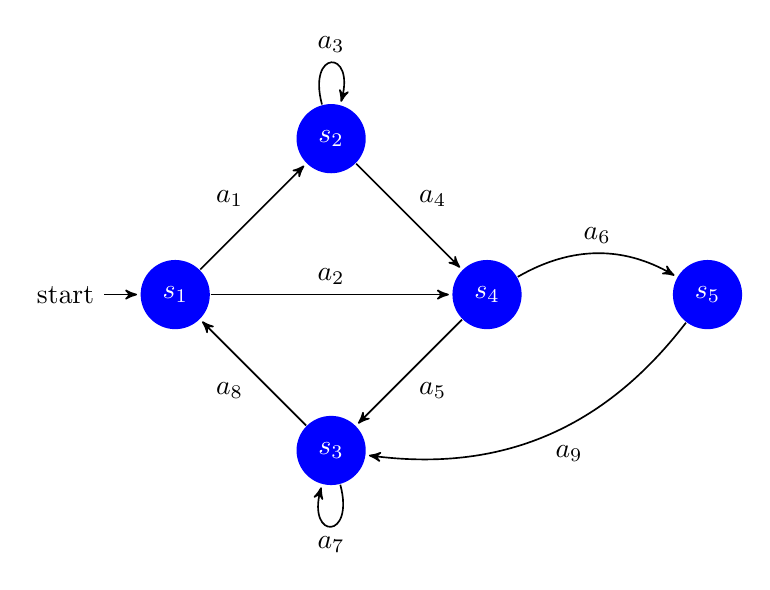
\begin{tikzpicture}[->,>=stealth',shorten >=1pt,auto,node distance=2.8cm, semithick]
  \tikzstyle{every state}=[fill=blue,draw=none,text=white]

  \node[initial,state] (A)                    {$s_1$};
  \node[state]         (B) [above right of=A] {$s_2$};
  \node[state]         (D) [below right of=A] {$s_3$};
  \node[state]         (C) [below right of=B] {$s_4$};
  \node[state]         (E) [right of=C]       {$s_5$};

  \path (A) edge              node {$a_1$} (B)
            edge              node {$a_2$} (C)
        (B) edge [loop above] node {$a_3$} (B)
            edge              node {$a_4$} (C)
        (C) edge              node {$a_5$} (D)
            edge [bend left]  node {$a_6$} (E)
        (D) edge [loop below] node {$a_7$} (D)
            edge              node {$a_8$} (A)
        (E) edge [bend left]  node {$a_9$} (D);
\end{tikzpicture}

\end{document}